\section{Teaching Programming with Games}
\label{sec:teachProgWithGames}
We have not been able to find many games that try to teach programming fundamentals. Carnage Heart for the original PlayStation is one of the few that exist. In the game, the player has to create a robot that has to fight other robots in a war. However, the robot cannot be controlled directly, instead the player has to program its behavior using a grid of icons, as seen on \autoref{fig:carnageheartsoftware}.

\begin{figure}[h]
  \centering
    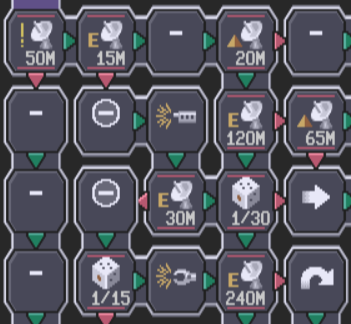
\includegraphics[width=0.5\textwidth]{img/CarnageHeartSoftware.png}
  \caption{Screenshot of the programming interface in Carnage Heart.\cite{carnageheartsoftware}}
  \label{fig:carnageheartsoftware}
\end{figure}

Carnage Heart teaches only basic programming constructs, but do not present them as such. Instead the player is presented with a set of rules, which are much like the rules of programming, and are told to create what is basically an AI for the robot.\\

Another example of a game trying to teach programming is CodeCombat. \cite{codecombat} CodeCombat is a browser-based game, that tries to teach JavaScript programming by making the player write code to play an RPG. The player plays as a wizard, and the programming is represented as magic spells in the game. The player is programming an AI for a knight, that has to fight a variety of monsters. Control of the knight includes movement and attack as well as conditions such as attack if the enemy is in range.
Although CodeCombat is a game, it is very explicit in its teaching.\todo{Why?} Tools such as Codecademy provide the same kind of programming guides as CodeCombat, but without the gaming aspect.\cite{codecademy}\\

Microsoft has released a game for teaching children programming called Kodu Game Lab. \cite{kodu} Kodu Game Lab is a free game on the PC and can be bought for $\$4.99$ on the Xbox 360 marketplace. This means, that the game is available to most children. In the game, the player starts with a small world, a square of grass. The player can then add objects and program them to do what the player wants. It is possible to make an object react to other objects, e.g. eat them. The programming interface, see figure \autoref{fig:kodu}, in Kodu Game Lab is very simple, and visually illustrates what will happen. 

\begin{figure}[h]
  \centering
    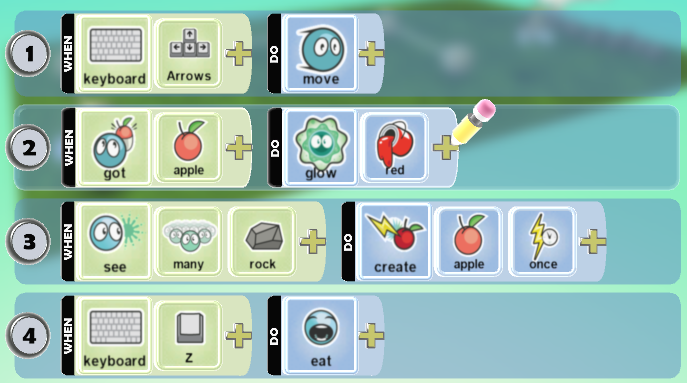
\includegraphics[width=\textwidth]{img/kodu.png}
  \caption{Screenshot of the programming interface in Kodu Game Lab.}
  \label{fig:kodu}
\end{figure}\todo{source}

The way Carnage Heart and Kodu Game Lab approach teaching basic programming constructs is very relevant to our project, and could be a source of inspiration when we need to design our own game.